% \chapter{Présentation du projet}
    \section{Définition générale du besoin : l'Interpréteur LIR}
L’Interpréteur LIR est un interpréteur d’un langage de programmation
simple, il sera nommé LIR pour Langage IUT de Rodez.
Un interpréteur est un automate enchaînant les tâches suivantes :
analyse lexico-syntaxique d’une ligne de commande puis interprétation.
\\Une ligne entrée par un utilisateur sera donc : soit une commande à
exécuter immédiatement, soit une ligne de programme à mémoriser pour
une exécution ultérieure. Une ligne de programme se distinguera d'une
ligne de commande par le fait qu'elle sera toujours précédée d'un
"numéro d'ordre" appelé aussi "étiquette".

\section{Cahier des charges}
Le document en annexe fourni par la maîtrise d’ouvrage (MOA) définit
l’interpréteur attendu avec les éléments du Langage IUT de Rodez, la
syntaxe des instructions de programmation et des commandes générales
attendues dans le logiciel final. Le document précise également le
comportement attendu de l’interpréteur lors de son utilisation suivi
d’un exemple d’une session sous cet interpréteur LIR.

\section{Définitions et acronymes}
\paragraph{Analyse syntaxique :}
La vérification de la conformité aux contraintes syntaxiques
définies par une grammaire.

\paragraph{Analyse lexicale :}
L’identification des éléments du vocabulaire d’un langage dans
une description textuelle (scanning) et la recherche des unités
lexicales (lexèmes).

\paragraph{Grammaire :}
Contraintes syntaxiques définissant les constructions correctes
(autorisées) d’un langage.

\paragraph{Interpréteur :}
Programme capable d’analyser les instructions d’un langage
(évolué) et de les exécuter directement.

\paragraph{Langage :}
Outil de description et d’expression.

\paragraph{Langage IUT de Rodez (LIR)}

\paragraph{Sémantique :}
Étude du sens des unités linguistiques et de leurs combinaisons.
\\Aspect de la logique qui traite de l'interprétation et de la
signification des systèmes formels, par opposition à la syntaxe, entendue
comme l'étude des relations formelles entre formules de tels systèmes
(d’après le dictionnaire Larousse).

\paragraph{Syntaxe :}
Partie de la grammaire qui décrit les règles par lesquelles les unités
linguistiques se combinent en phrases. En logique, étude des relations
formelles entre expressions d'un langage (d’après le dictionnaire
Larousse).
\\Aussi, la syntaxe est spécifiée par des grammaires et des notations
formelles.

\paragraph{Vocabulaire :}
Symboles de base utilisés dans un langage.

\section{Charte de projet}
\subsection{Objectifs du projet}
Réaliser un interpréteur capable d'exécuter un script ou une série
d'instructions dans le langage LIR avec les outils et connaissances
et mis à disposition par l’IUT de Rodez.

\subsection{Périmètre du projet}
Ce projet est doit être mené jusqu'à obtention d’un interpréteur
capable d’exécuter toutes les commandes précisées dans le cahier des
charges fourni.

\subsection{Demandes hors périmètre}
Il n’y a pas de demandes hors périmètre.

\subsection{Principaux livrables identifiés}
\paragraph{Livrables :} plan projet, dossier de projet, CD (de
préférence un dossier compressé plutôt qu’un CD) contenant les codes
exécutables les fichiers de données, les codes sources et la version
numérique du dossier et le manuel utilisateur.

\paragraph{Définition du cadre}
\subparagraph{Coût :} À définir par le chef de projet (P. Debas).
\subparagraph{Délais :} Deux dates butoirs identifiées.
\begin{itemize}
    \item Remise du projet le vendredi 28 mai 2021.
    \item Soutenance du projet la semaine du 7 juin 2021.
\end{itemize}

\subparagraph{Qualité :}
Projet codé en Java dans les respects des conventions et bonnes
pratiques.

\subsection{Les acteurs du projet}

\begin{center}
    \begin{tabular}{rl}
        L'équipe MOE :        & N. CAMINADE, S. COURTIOL, \\
        & P. DEBAS, H. DEXTER,      \\
        & L. VABRE                  \\
        La MOA :              & F. Barrios                \\
        Le contrôle qualité : & F. Barrios et J. Accot    \\
    \end{tabular}
\end{center}

\subsection{Autres moyens et ressources}
Pas de moyens ou ressources supplémentaires.

\subsection{Conditions d’acceptation}
Pas d’exigence ou de contraintes supplémentaires.

\subsection{Principaux risques identifiés et politique de gestion des risques}
Si possible tous les membres du groupe auront les mêmes droits sur
les fichiers communs. En conséquence chaque membre du groupe ne doit
pas donner des droits sur ces fichiers à une personne extérieure au
projet (autre que MOA). Cf. Gestion de la configuration (produit par
S. Courtiol).
\\Des sauvegardes du dépôt GitHub (contenant toutes les données du
projets) seront effectuées régulièrement (fréquence à définir) par le
gestionnaire de configuration. Toutes données qui ne sont pas dans le
dépôt sont à la responsabilité de chacun. Cf. Gestion de la
configuration (produit par S. Courtiol).

\section{Étude générale du besoin}
\paragraph{Diagramme de cas d'utilisation général de l'Interpréteur LIR}
comprenant un acteur (le programmeur) et deux cas d'utilisation
identifiés comme suit :
\\

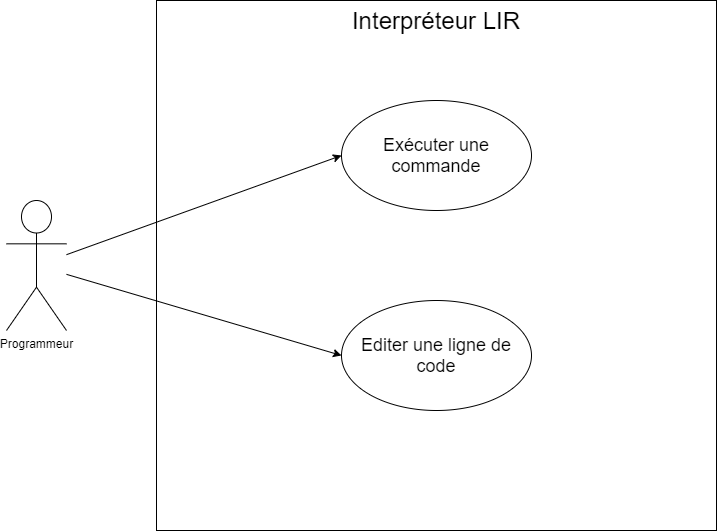
\includegraphics[width=\linewidth]{./img/DiagrammeCasUtilisation.png}

\subsection{Les acteurs}
\paragraph{Programmeur :} % TODO à détailler
Personne utilisant l'interpréteur.

\subsection{Résumés de cas d'utilisation}
\subsubsection{\Large --- Exécuter une commande}

    \subparagraph{Acteurs}
    Programmeur : il entre une commande à faire exécuter immédiatement par l'interpréteur.

    \subparagraph{Objectifs}
    Exécuter la commande entrée dans l'interpréteur.

    \subparagraph{Pré-Conditions}
    L'interpréteur LIR est lancé et le curseur est derrière l'invite.

    \subparagraph{Post-Conditions}
    La commande est exécutée et un résultat ou un feedback est affiché.

    \subparagraph{Scénario nominal (grandes étapes)}
        \begin{enumerate}
            \item Le programmeur écrit derrière l'invite une ligne de commande.
            \item Le programmeur valide cette commande.
            \item L'interpréteur effectue une analyse lexico-syntaxique.
            \item L'interpréteur interprète la ligne de commande.
        \end{enumerate}

    \subparagraph{Scénarios d'échec}
        \subparagraph{Point 3 du scénario nominal :} la syntaxe de la ligne écrite est incorrecte.
        \begin{itemize}
            \item Un message d'erreur explicite informe le programmeur.
            \item Retour au point 4 du scénario nominal.
        \end{itemize}

        \subparagraph{Point 4 du scénario nominal :} la commande conduit à une erreur d'exécution.
        \begin{itemize}
            \item Un message d'erreur explicite informe le programmeur.
            \item Retour au point 4 du scénario nominal.
        \end{itemize}

%\end{document}

\subsubsection{\Large --- Éditer une ligne de code}


\title{Résumé de cas d'utilisation --- Éditer une ligne de code} % à remplacer


        \subparagraph{Acteurs}
            Programmeur : Il écrit ou modifie une ligne de code dans un
            programme à faire exécuter par l'interpréteur.

        \subparagraph{Objectifs}
            Écrire une une ligne de code dans nouveau programme ou un
            existant afin d'exécuter ou de sauvegarder ce programme.

        \subparagraph{Pré-conditions}
                Le curseur est derrière l'invite suivi d'une étiquette correspondant
                au numéro de la ligne de code à éditer.

        \subparagraph{Post-conditions}
                Le code source édité est prêt à être exécuté, abandonné ou sauvegardé,
                selon l'intention du programmeur.

        \subparagraph{Scénario nominal (grandes étapes)}
            \begin{enumerate}
                \item Le programmeur écrit une instruction ou commande par ligne de code, en la faisant précéder de son étiquette.

                \item Le programmeur consulte le code déjà écrit à tout moment avec la
                      commande \verb|liste|. Selon la syntaxe choisie, l'interpréteur
                      affiche la plage demandée ou la totalité des lignes de code
                      du programme dans l'ordre croissant des étiquettes.

                \item Le programmeur consulte la liste des identificateurs déclarés et
                      leurs valeurs en entrant la commande \verb|defs|.

                \item Au besoin, le programmeur efface une ou plusieurs lignes avec la
                      commande \verb|efface|.

                \item Au besoin, le programmeur efface les lignes de code et identificateurs mémorisés et commence un nouveau code avec la commande \verb|debut|.
            \end{enumerate}

        \subparagraph{Scénarios d'échec}

            \paragraph{Point 2 du scénario nominal :} Aucune ligne de code n'est écrite ou
            la plage de code à afficher n'est pas correcte.
            \begin{itemize}
                \item L'interpréteur en avise le programmeur au moyen d'un message d'erreur.
                \item Retour au point 1.
            \end{itemize}

            \paragraph{Point 3 du scénario nominal :} Aucun identificateur n'a encore été
            déclaré.
            \begin{itemize}
                \item L'interpréteur affiche un message informant le programmeur.
                \item Retour au point 1.
            \end{itemize}

            \paragraph{Point 4 du scénario nominal :} La plage de ligne à effacer est
            incorrecte.
            \begin{itemize}
                \item Un message d'erreur en informe le programmeur
                \item Retour au point 1.
            \end{itemize}


\subsection{Récits d'utilisation (user stories)}
Les récits d'utilisation %TODO déf
\\Des récits d'utilisation ont été rédigés pour chaque commande et instruction.

